\exam{2021}
\begin{problem}{Poisson process}
Let $P_1$ and $P_2$ be two independent Poisson processes with rates 
$\lambda_1$ and $\lambda_2$ . Let $N_{t,i}$ be the number of arrivals of process $P_i$ in [0, t], for i = 1, 2. Show that:
\begin{align*}
    \lambda_2^k P(N_{t,1} = N_{t,2} + k) 
    &=\lambda_1^k P(N _{t,2} = N_{t,1} + k)
\end{align*}
\end{problem}

\begin{problem}{Markov Chains}
Give an example of a DTMC with 6 states, where some states have period 2 and others have period 3, while not all states are recurrent. Explain your answer. What is the maximum number of non-zero entries in \( P \) for such a chain? Explain.
\end{problem}
\begin{solution}
    \begin{figure}[h!]
        \begin{center}
            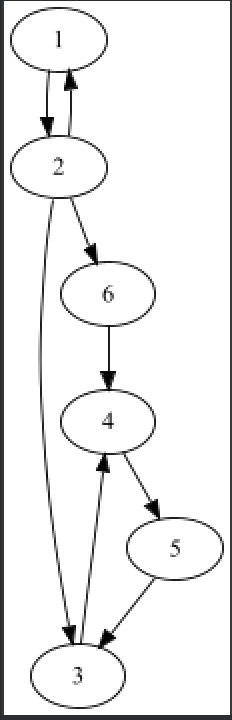
\includegraphics[height=0.5\textwidth]{img/21.2.png}
        \end{center}
        \caption{DTMC with 6 states. 1,2 have period 2, 3-5 period 3 and 6 not recurrent}
    \end{figure}
\end{solution}
States 1-2 communicate with period of 2. States 3-5 communicate with period of 3. State 6 does not go anywhere to ensure that it is not recurrent. Writing out the matrix P gives us six non-zero entries.\\
\begin{problem}{Markov Chains}
Let \( Y_i \), for \( i \geq -1 \), be an infinite set of independent random variables with \( P [Y_i = -1] = P [Y_i = 0] = P [Y_i = 1] = \frac{1}{3} \). Define \( X_n = Y_{n-1} + Y_n \) for \( n \geq 0 \). Is \( (X_n)_{n \geq 0} \) a DTMC? If so, give its transition matrix \( P \); if not, explain why.
\end{problem}

\begin{problem}{Markov Chains}
Consider two independent Poisson processes \( P_1 \) and \( P_2 \) with rates \( \lambda_1 \) and \( \lambda_2 \). Assume we have an infinite bag, and whenever an arrival occurs of process \( P_1 \) we add a ball to the bag. If an arrival occurs of process \( P_2 \), we remove half of the balls from the bag, that is, we remove \( \lceil k/2 \rceil \) balls if the bag contains \( k \) balls (\( \lceil x \rceil \) rounds \( x \) to the smallest integer larger than or equal to \( x \)). Let \( X_t \) be the number of balls in the bag at time \( t \). Argue that \( (X_t)_{t \geq 0} \) is an irreducible CTMC. Given \( \lambda_1 \), how large must \( \lambda_2 \) be such that this CTMC is positive recurrent? Explain your answer.
\end{problem}

\begin{problem}{Applications}
Consider 2 queueing systems. The first is an M/M/1 queue with arrival rate \( \lambda = 0.3 \) and mean service time equal to 2. The second is a Jackson network with \( M = 1 \), \( \mu_1 = 4 \), and \( p_{1,1} = \frac{1}{3} \). How should we set \( \lambda_0 \) such that the queue length distribution is the same in both queueing systems? Explain.
\end{problem}

\begin{problem}{Applications}
Consider an Erlang-C system with \( C \) servers, i.e. an M/M/C/C+Q queue with \( Q = \infty \). Assume we know that on average \( k \) jobs are waiting in the waiting room to enter a server. Does the mean time that a customer spends in the system depend on \( C \), \( k \), or both \( C \) and \( k \)? Explain.
\end{problem}
